% Section: fixed fees, entry and other externalities (input by mfg/paper/main.tex); numbers from numbers_ext.tex
\section{Fixed fees, entry and other externalities}\label{sec:ext}
Section~\ref{sec:stake} left three questions open: who pays for the subsidy that the efficient charge contains when carriers are few, what the subsidy and the charge do to the number of carriers, and what changes when delivery traffic causes costs other than in-zone delay.

\subsection{Recovering the subsidy with a fixed fee}\label{sec:fees}
Let the city post a charge $u$ per delivery and, in addition, collect a fee $T_i$ from carrier $i$. Call the fee \emph{lump-sum} if it is fixed before carriers choose their plans: it may depend on the carrier's identity, its licensed fleet or the plan the city is aiming at, but not on the deliveries the carrier actually makes.

\begin{proposition}[Lump-sum fees]\label{prop:fee}
Fix the set of $N$ carriers, a charge $u$ and outside options $\underline\pi_i$.
\begin{enumerate}
\item[(a)] With lump-sum fees the Nash equilibria are those without fees. Deliveries, consumer surplus, congestion cost and welfare are unchanged; the fees move $\sum_iT_i$ from carriers to the city.
\item[(b)] All carriers stay in the market iff $\pi_i(u)-T_i\ge\underline\pi_i$ for every $i$, where $\pi_i(u)$ is carrier $i$'s equilibrium profit net of the charge. Fees with $\sum_iT_i=D$ and participation exist iff $\sum_i(\pi_i(u)-\underline\pi_i)\ge D$; for the deficit $D=-R$ of the charge and $\underline\pi_i=0$ this reads $\Pi_{\rm op}-\mathrm{CC}\ge0$, operating profit net of the delay cost at the target.
\item[(c)] A fee that recovers the \emph{realised} deficit, $T_i=-\ip{u}{Q}/N$, is not lump-sum. Carrier $i$ then faces the charge $(1-\tfrac1N)u$ on its own deliveries, and in the one-zone case of Proposition~\ref{prop:marketpower} the Nash aggregate under $u=u_N^*<0$ falls below $Q^\opt$.
\end{enumerate}
\end{proposition}
\emph{The proof is in Appendix~\ref{app:proofs}.}

The proposition is elementary; for the city, (b) and (c) say that the fee must be computed from the target plan, not from the books after the fact, and must leave each carrier its outside option. Table~\ref{tab:fees} applies it to the market-power rule of Section~\ref{sec:stake} with outside option zero. At $N=6$ the deficit is \FeeSixDef\,\% of welfare (median) and the charge is a subsidy in \FeeSixSub\,\% of zone-hours; recovering it takes \FeeSixShare\,\% of carrier profit (range \FeeSixShareMin--\FeeSixShareMax\,\%). A flat fee per carrier leaves some carrier with a loss in every instance (participation in \FeeSixFlatOK), a fee in proportion to the licensed fleet in \FeeSixFleetOK{} instances; carrier-specific fees exist in \FeeSixAggregateOK{} instances, the exceptions being \FeeAggFailCities, where the subsidy exceeds total carrier profit. At $N=24$ the fee takes \FeeTwentyFourShare\,\% of profit and a flat fee keeps every carrier in \FeeTwentyFourFlatOK{} instances; at $N=192$ the charge is a subsidy only in some cities and the fee takes \FeeOneNinetyTwoShare\,\% (participation \FeeOneNinetyTwoFlatOK{} flat); at $N=1536$ the charge raises revenue and no fee is needed. After the fee, carriers keep \FeeSixKept\,\% of their no-charge profit at $N=6$ (\FeeTwentyFourKept\,\% at $N=24$): the subsidy and the fee together transfer the Cournot rent to buyers, and for $N\le192$ no fee scheme leaves every carrier with at least its no-charge profit in any instance. Recovering the realised deficit instead (part (c)) costs \FeeSixEpLoss\,\% of optimal welfare at $N=6$, small because the residual subsidy is still $(1-\tfrac16)u$.



So the subsidy is budget-balanceable with participation only with carrier-specific fees at $N=6$, and with simple fees from about $N=192$ on, where it is small. With a fixed set of carriers this is about distribution; it stops being so when carriers can leave or enter.

\subsection{Entry and exit}\label{sec:entry}
\paragraph{Model} Segment $\theta$ has $k_\theta$ identical carriers that share its fleet budget $B_\theta$ (Section~\ref{sec:data}); the fleet is a pool of drivers and vans calibrated from demand, so entry adds firms, not vehicles. Each carrier pays a fixed cost $F_\theta$ per day (depot, licence, management; vehicle costs are in the tour cost). Counts are real numbers, a continuous approximation of the integer count; a segment whose single carrier cannot cover $F_\theta$ leaves the market. A \emph{free-entry equilibrium} under a charge rule is a Nash equilibrium with $\pi_\theta/k_\theta-T_\theta=F_\theta$ for every active segment, $\pi_\theta$ the segment's profit net of the charge and $T_\theta$ its fee per carrier. Welfare is $\SW-\sum_\theta k_\theta F_\theta$.

\begin{proposition}[Free entry]\label{prop:entry}
\begin{enumerate}
\item[(a)] At every free-entry equilibrium, under any charge and lump-sum fees, welfare net of fixed costs equals $\mathrm{CS}+R+\sum_\theta k_\theta T_\theta$: consumer surplus plus the city's net revenue. Of two rules that produce the same aggregate, the one with the larger net revenue has the larger welfare.
\item[(b)] One zone, $N$ identical carriers, slack budget, charge $u$, no fee. Every carrier delivers $s=(F/m)^{1/2}$ whatever $u$, and the free-entry number is $N^*(u)=(\alpha-u)/(mF)^{1/2}-1$. Under no charge $N_a=\alpha/(mF)^{1/2}-1$; under the observation-only rule $N_b=Q_b/s$ with $Q_b=(\alpha-ms)/(m+\kappa)$; under Pigou minus market power ($u=u^*_N$ of Proposition~\ref{prop:marketpower} with $N$ endogenous) $N_c=Q^\opt/s$; with the fee $T=-u Q^\opt/N$ recovering a subsidy, $N_d=\kappa(Q^\opt)^2/F$, smaller than $N_c$ exactly when the charge is a subsidy ($N_c<m/\kappa$).
\item[(c)] (Excess entry.) In (b) with $u=0$, welfare decreases in $N$ at $N_a$: a planner who could limit entry, but not change Cournot conduct, would admit fewer carriers.
\item[(d)] (Second best, one-zone linear case.) In (b), welfare net of fixed costs as a function of a constant charge $u$ is maximised at $u=\kappa Q_b$, the observation-only fixed point; the market-power term of $u^*_N$ is absent, and $u^*_N$ with endogenous $N$ gives lower welfare.
\end{enumerate}
\end{proposition}
\emph{The proof is in Appendix~\ref{app:proofs}.}

Part (c) is the business-stealing result of \citet{MankiwWhinston1986}; parts (a), (b) and (d) are short computations in the same model. The literature on taxes under free-entry oligopoly finds that the optimal specific tax departs from the Pigou level by a term of either sign that depends on the curvature of demand and costs \citep{Konishi1990,KatsoulacosXepapadeas1995,Hamada2022}. Part (d) holds in the one-zone linear case only: output per carrier is pinned down by $F$ alone, a charge changes only the number of carriers, and the departure is zero. The congestion-pricing literature with market power \citep{Brueckner2002,PelsVerhoef2004} gives the fixed-$N$ counterpart, a toll below the congestion cost and possibly negative, which is Proposition~\ref{prop:marketpower}, a finite-$N$ analogue of those results. With $N$ endogenous the market-power subsidy no longer buys output per carrier; it buys entrants.

\paragraph{Calibration of $F$} $F_\theta$ is not observed; we set it so that the no-charge free-entry count lies between $k_0$ and $k_0+1$ carriers per segment (the geometric mean of the profit per carrier at $k_0$ and $k_0+1$), for $N_0=6k_0\in\{6,24,192\}$ (three seeds, \EntInst{} city-seed pairs), and sweep $N_0\in\{12,48,96,384\}$ on seed 0. A smaller $N_0$ means a larger fixed cost. Zero-profit residuals are below $10^{-5}$ of $F$ except for the market-power rules, where \EntConv{} runs reached $10^{-4}$ and the rest stopped after 80 rounds (residual up to \EntErrMax{} of $F$, identity of Proposition~\ref{prop:entry}(a) to \EntIdErr{} of welfare); no reported sign depends on them.



\paragraph{Results} Table~\ref{tab:entry} and Figure~\ref{fig:entry}. \emph{The subsidy attracts entrants.} Under Pigou minus market power the count rises to \EntSixPmN{} at $N_0=6$ and \EntTwentyFourPmN{} at $N_0=24$, and welfare net of fixed costs changes by \EntSixPmdSW\,\% and \EntTwentyFourPmdSW\,\% against no charge (ranges \EntSixPmdSWMin{} to \EntSixPmdSWMax\,\% and \EntTwentyFourPmdSWMin{} to \EntTwentyFourPmdSWMax\,\%): the rule that gained \WSixPmdSW\,\% with six fixed carriers loses in every instance once entry responds, because the subsidy pays for fixed costs instead of output. \emph{The recovery fee drives exits.} With the fee the count falls to \EntSixPmfeeN{} at $N_0=6$ (median \EntSixPmfeeAct{} of six segments stay; the market closes in \EntSixPmfeeClosed{} instances) and to \EntTwentyFourPmfeeN{} at $N_0=24$ (\EntTwentyFourPmfeeAct{} segments). The fee raises the cost of being a carrier by about the subsidy each one receives (Proposition~\ref{prop:entry}(b)). Because free entry is excessive (below), the exits can raise welfare: the fee rule beats no charge in \EntSixPmfeeBeatsNone{} instances at $N_0=6$ and \EntTwentyFourPmfeeBeatsNone{} at $N_0=24$ (median \EntSixPmfeedSW{} and \EntTwentyFourPmfeedSW\,\%, ranges \EntSixPmfeedSWMin{} to \EntSixPmfeedSWMax\,\% and \EntTwentyFourPmfeedSWMin{} to \EntTwentyFourPmfeedSWMax\,\%); it acts as an uncontrolled entry restriction whose outcome ranges from closing the market to a large gain. \emph{The observation-only charge is safe and close to the second best.} It changes the count little (\EntSixObsN, \EntTwentyFourObsN, \EntOneNinetyTwoObsN), raises welfare and beats the market-power rule in every instance, and is the best of the scalings $\theta\in\{0.5,1,1.5\}$ in \EntSixObsBest, \EntTwentyFourObsBest{} and \EntOneNinetyTwoObsBest{} instances: the one-zone result of Proposition~\ref{prop:entry}(d) holds approximately, less so with many carriers. The gains are small (\EntSixObsdSW, \EntTwentyFourObsdSW{} and \EntOneNinetyTwoObsdSW\,\%) because the calibrated congestion is weak. The $F$ sweep in Figure~\ref{fig:entry} shows the same ordering at every $N_0$; the fee rule's median changes sign between $N_0=12$ and $N_0=24$.

\emph{Excess entry.} Scaling the no-charge free-entry counts by $\lambda$ (at least one carrier per segment, conduct unchanged), welfare net of fixed costs is largest at one carrier per segment for $N_0=6$, at $\lambda=\EntTwentyFourLamBest$ ($\EntTwentyFourNLam$ carriers) for $N_0=24$ and at $\lambda=\EntOneNinetyTwoLamBest$ ($\EntOneNinetyTwoNLam$ carriers) for $N_0=192$, gains of \EntSixMwGain, \EntTwentyFourMwGain{} and \EntOneNinetyTwoMwGain\,\% of welfare; entry is excessive in every instance. Cournot withholding is small once a segment has a few carriers, while each carrier's fixed cost is not. This is the largest welfare effect in this section and it is not a pricing effect: per-delivery charges cannot remove it, and the city's other instrument, a fee on entry, needs the information on profits discussed in Section~\ref{sec:fees}.

\begin{figure}[t]
\centering
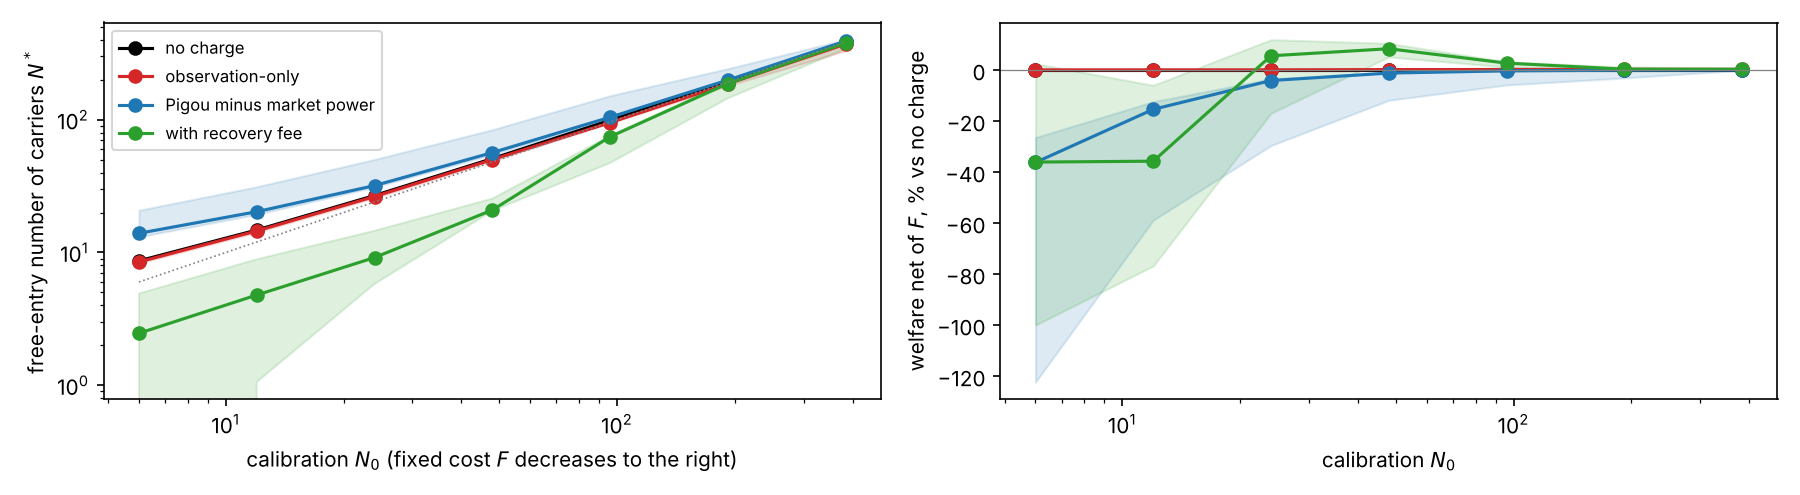
\includegraphics[width=0.88\textwidth]{mfg_entry.png}
\caption{Free entry against the calibration $N_0$ (medians and interquartile ranges; $N_0\in\{6,24,192\}$ over three seeds, the sweep points on seed 0). Left: free-entry number of carriers. Right: welfare net of fixed costs, \% change against no charge.}\label{fig:entry}
\end{figure}

\paragraph{What is not modelled} Fixed costs are not sunk (entry and exit are free, so $N^*$ is a long-run object) and are common within a segment; with heterogeneous fixed costs inframarginal carriers keep rents and the identity of Proposition~\ref{prop:entry}(a) holds only at the margin. The fleet of a segment is fixed; entrants with their own vehicles would add capacity. The count is continuous; the integer constraint \citep{MankiwWhinston1986} moves $N^*$ by less than one carrier per segment.

\subsection{Emissions, noise and through-traffic}\label{sec:extern}
So far the only externality is the delay that delivery vehicles impose on each other while serving a zone; driving between zones is priced only through the tour's own cost. We add emissions, noise and the delay that driving between zones imposes on other traffic as a cost $E_j$ per tour, linear in its vehicle-km:
\[
E_j=\sum_{\text{legs}}\ell_{\rm leg}\big(e_{\rm air}+e_{\rm clim}+e_{\rm noise}\big)+\sum_{\text{legs}}t^0_{\rm leg}\,g(h_{\rm leg})+\sum_{\text{stops}}\ell_{\rm stop}\big(e_{\rm air}+e_{\rm clim}+e_{\rm noise}\big),
\]
with $e_\cdot$ in USD per vehicle-km and welfare $\SW_{\rm ext}=\SW-\sum_i\ip{E_i}{y_i}$. A leg's length $\ell_{\rm leg}$ is the length of the fastest path between the two zone nodes on the major-road graph of the processed city data (the same paths as the travel-time matrix of Section~\ref{sec:data}, reproduced to $10^{-7}$), plus an access drive of 120\,s at each end. The driving between the drops of one stop, $\ell_{\rm stop}=0.7124(A_z\,\mathrm{lot})^{1/2}$, is the Beardwood--Halton--Hammersley length of a tour through $\mathrm{lot}$ points spread over the zone's area $A_z$ \citep{BHH1959}. Through-traffic delay is the marginal external delay of one vehicle under the BPR curve \citep{BPR1964}: a vehicle on a link with free-flow time $t^0$ at congestion level $c$ adds $\beta c\,t^0$ hours of delay to all others, so $g(h)=\mathrm{pce}\,\beta\,\mathrm{cong}(h)\,\mathrm{VOT}$ per free-flow hour of the leg, at the hourly congestion level of Section~\ref{sec:data}. It is charged on inter-zone legs only; delay inside a zone is the $\kappa$ term already in the model. Table~\ref{tab:extparams} lists the values.



\begin{proposition}[Charges for linear tour externalities]\label{prop:extcharge}
Let tour $j$ of carrier $i$ cause the external cost $E_{ij}$, and let $Q'$ be the aggregate of an extended social optimum (maximiser of $\SW_{\rm ext}$).
\begin{enumerate}
\item[(a)] A charge $E_{ij}$ per tour (a distance charge) plus $\kappa\odot Q'$ per delivery makes the mean-field equilibrium an extended optimum; for $N$ identical carriers, a charge $E$ per tour plus $(\kappa-\tfrac mN)\odot Q'$ per delivery makes the Nash equilibrium one.
\item[(b)] If the external cost is additive over deliveries, $E_i=L_i^\top e$ for a common $e\in\R^d$, the per-delivery charge $\kappa\odot Q'+e$ alone does the same in the mean field.
\end{enumerate}
\end{proposition}
\emph{The proof is in Appendix~\ref{app:proofs}.}

Vehicle-km are not proportional to deliveries, so (b) holds only approximately. We compute, in the mean field, the exact rule of (a); the \emph{matched} per-delivery charge that reproduces $Q'$ (damped iteration as in Section~\ref{sec:stake}); and the simple rule $u=\kappa\odot Q'+\bar e$, with $\bar e_k$ the external cost of the tours delivering at $k$ per delivery made there; at finite $N$, the market-power rule with these terms.



\paragraph{Results} Table~\ref{tab:extern} and Figure~\ref{fig:extern}. A delivery drives \ExtVkmDel{} vehicle-km (median; \ExtVkmInShare\,\% of it inside the delivery zones) and causes \ExtPerE{} USD of external cost beyond in-zone delay (city medians \ExtPerEMin--\ExtPerEMax), \ExtShareFee\,\% of the delivery fee (\ExtShareFeeMin--\ExtShareFeeMax\,\%). Through-traffic delay is \ExtShareCong\,\% of it; emissions are \ExtPerAir{} (air) and \ExtPerClim{} (climate) USD per delivery and noise \ExtPerNoise. The external cost is \ExtRatioKQ{} times the in-zone congestion charge $\kappa Q$ (city medians \ExtRatioKQMin--\ExtRatioKQMax). This is the main finding of the extension and a negative one for the model of the earlier sections: the congestion term that the model prices, the delay among delivery vehicles while they serve a zone, is the smaller part of the congestion they cause.

\emph{The charge.} The matched per-delivery charge is \ExtChargeMatch{} USD per delivery against \ExtChargeCong{} for the congestion-only Pigou charge (median ratio \ExtChargeRatio, by city \ExtChargeRatioMin--\ExtChargeRatioMax). At the extended optimum deliveries fall by \ExtDQ\,\% and vehicle-km by \ExtDVkm\,\% (\ExtDVkmPerDel\,\% per delivery: carriers switch to tours with fewer km per drop). \emph{Welfare.} Without a charge the market loses \ExtLossNone\,\% of the optimal welfare of Section~\ref{sec:stake} to the extended optimum (above 20\,\% in New Delhi, Mumbai and London); the congestion-only Pigou charge recovers \ExtGainCongShare\,\% of this gap (at most \ExtGainCongShareMax\,\%), the matched per-delivery charge all but \ExtLossMatch\,\% (at most \ExtLossMatchMax\,\%), and the simple rule $\kappa\odot Q'+\bar e$ all but \ExtLossEbar\,\%: averaging the cost of a tour over its deliveries does not reproduce the optimal aggregate (deliveries \ExtEbarDQ\,\% and vehicle-km \ExtEbarDVkm\,\% against the extended optimum). Zone-hour charges therefore suffice for these externalities if they are set to match the right aggregate; a distance charge adds little. With few carriers market power still dominates: at $N=6$ the losses are \ExtSixNone\,\% (no charge), \ExtSixPmCong\,\% (market-power rule, congestion only), \ExtSixPmMatch\,\% (extended, per delivery) and \ExtSixPmTour\,\% (extended, with distance charge); at $N=1536$ they are \ExtBigNone, \ExtBigPmCong, \ExtBigPmMatch{} and \ExtBigPmTour\,\%.

\emph{Sensitivity.} European values everywhere: \ExtSensEuE{} USD per delivery, no-charge loss \ExtSensEuNone\,\%; Euro~4 air pollution and the EPA carbon value: \ExtSensHiE{} and \ExtSensHiNone\,\%; emissions and noise only: \ExtSensNoCongE{} and \ExtSensNoCongNone\,\%. Emissions and noise alone change the earlier conclusions very little; the through-traffic term carries the result, and its value of time (the driver wage applied to all traffic) is the weakest parameter of Table~\ref{tab:extparams}.

\emph{Exposure.} Assigning each leg's km to the zones its path crosses and each stop's km to its zone, delivery traffic puts \ExpVkmNone{} vehicle-metres per resident and day on the zones it touches (city medians \ExpVkmNoneMin--\ExpVkmNoneMax; \ExpThroughNone\,\% in zones that receive no deliveries), an air-pollution damage of \ExpAirNone{} USD per resident and year (at most \ExpAirMax). This exposure is far less even than the in-zone exposure of Section~\ref{sec:residents}: Gini \ExpGiniNone{} against \ExpBigGiniNone, and a top-to-bottom decile ratio of \ExpDtenNone, consistent with through traffic running on a few corridors. Across served zones it is positively but loosely rank-correlated with the in-zone exposure (Spearman \ExpCorrCong, city medians \ExpCorrCongMin--\ExpCorrCongMax). The extended charge cuts this exposure by \ExpVkmDTour\,\% (congestion-only Pigou: \ExpVkmDCong\,\%) but raises its Gini to \ExpGiniTour{} (higher in \ExpGiniUp{} instances); why the remaining traffic is more concentrated was not tested. Population is the only weight: there are no income or health data, and pollution damage is per vehicle-km, not modelled from concentrations.

\begin{figure}[t]
\centering
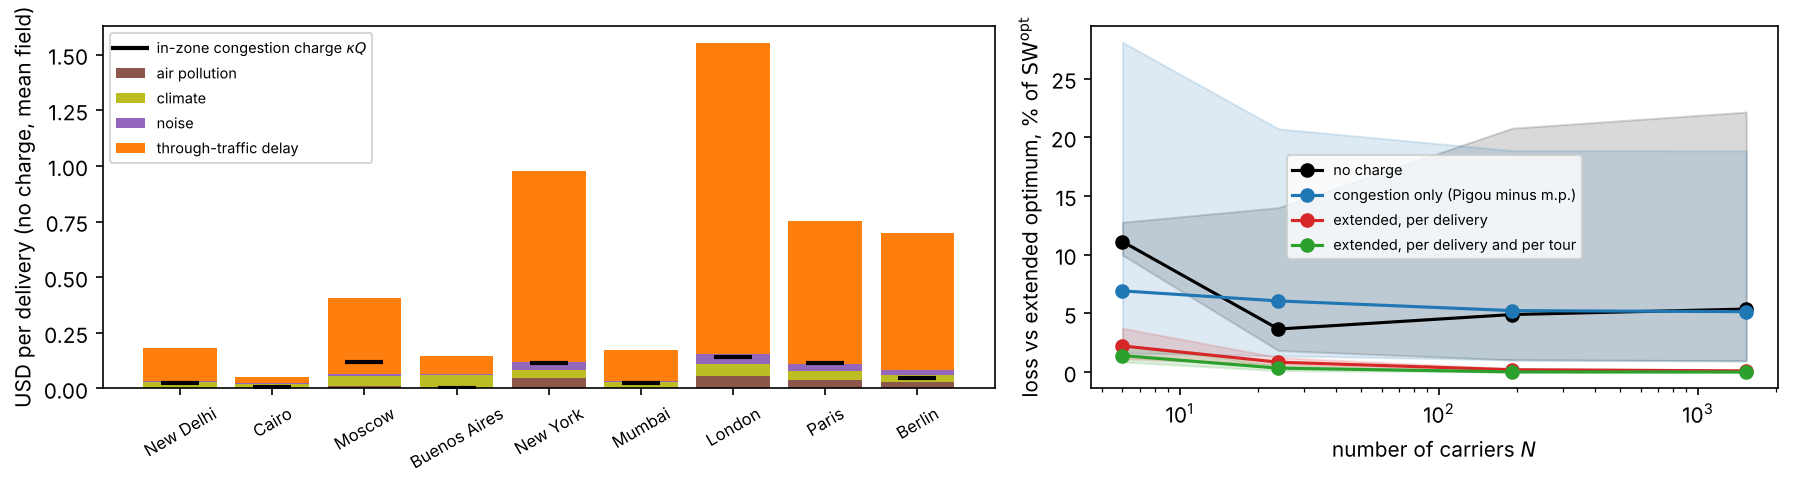
\includegraphics[width=0.88\textwidth]{mfg_extern.png}
\caption{Left: external cost per delivery by component and city (no charge, mean field, median of five seeds), with the in-zone congestion charge $\kappa Q$ (black). Right: welfare below the extended optimum against $N$ (\% of the optimal welfare of Section~\ref{sec:stake}; median and interquartile range over 45 instances).}\label{fig:extern}
\end{figure}
